\documentclass[fleqn, 11pt]{wlscirep}

\usepackage[strings]{underscore}
 
\usepackage[empty]{fullpage} % changes the margin
\usepackage{graphicx}
\usepackage{float}
\usepackage{nopageno}
\thispagestyle{empty}
\begin{document}
%Header-Make sure you update this information!!!!
\section*{\centering Resolving intercontinental plumes in global atmospheric models}
\textbf{Problem Statement}\\
Observations show that chemical plumes injected to the free troposphere (2-10 km altitude) by convection, volcanoes, or stratospheric intrusions can retain their identity as well-defined vertical layers for a week or more as they are transported on intercontinental scales.\cite{newell} \cite{thouret} \cite{heald} Eventually these plumes may entrain into the boundary layer, affecting air quality in continents downwind. Global atmospheric models fail to reproduce these plumes due to rapid numerical dissipation, even when using high-order transport algorithms.\cite{rastig} This problem affects the ability of the models to represent the long-range transport, radiative effects, nonlinear evolution, and surface impacts of the plumes.\cite{wild} \cite{zhuang}\ \cite{eastham}\ \\ \\
\textbf{Background}\\
Plume dissipation in models is caused by numerical diffusion when solving the advection equation:
\begin{equation}
\frac{\partial C}{\partial t}=-\textbf{u}\bullet \nabla C
\end{equation}
where C is the chemical mixing ratio, t is time, u is the wind vector, and the gradient operator operates in the three spatial dimensions. Exact solution preserves the mixing ratio while translating it downwind.\cite{rastig} Numerical schemes in Eulerian models (fixed spatial coordinates) use high-order finite differencing of the partial derivatives and are highly accurate in steady flow, but break down in realistic sheared flow, as the plumes filament down to the grid scale where any scheme collapses to first-order (because gradients cannot be properly described). Lagrangian models (spatial coordinates moving with the wind) have no such numerical diffusion problem but are of limited value because they do not provide a continuous representation of the atmosphere and cannot simulate nonlinear processes.\cite{brasseurjacob} 

The obvious cure is to increase the Eulerian model grid resolution, $h$. However, this will increase in turn flow shear so that preservation of the plumes scales only as $h^{1/4-1/2}$.\cite{rastig}  Off-line chemical transport models (CTMs), where transport information is from a general circulation model (GCM) meteorological archive, are further limited by the resolution of that archive.  GCM development over the past decades has prioritized horizontal resolution to model cyclogenesis and fronts. Much less emphasis has been placed on vertical resolution. Current GCMs have horizontal resolutions of 10-50 km, and vertical resolutions of 0.5-1 km in the free troposphere. Simulations with the GEOS-Chem CTM using meteorological data from the NASA Goddard Earth Observing System (GEOS) GCM. show that a horizontal resolution of 50 km is sufficient to preserve 2-D (horizontal) plumes for over a week, but 3-D plumes dissipated within a few days due to inadequate vertical resolution.\cite{zhuang} \cite{eastham} 

In preliminary work, I compared vertical profiles of ozone measured from ozonesondes with a very-high-resolution simulation of tropospheric chemistry in the NASA GEOS GCM with cubed-sphere c720 horizontal resolution (about 12x12 km2) and with 72 layers in the vertical (approximately 500 m resolution). Figure\ref{fig:proposal} shows results for Trinidad Head in northern California, where biweekly measurements are available.\cite{WOUDC} Individual profiles show well-defined vertical layers that may be contributed by Asian pollution, boreal forest fires, and stratospheric intrusions. These layers are sufficiently thick that they remain apparent even when smoothed over the vertical resolution of the model (dashed lines). The model by contrast has very little vertical structure and completely misses the observed layers, even though it can successfully simulate the seasonal mean profile. This is symptomatic of the numerical diffusion problem.\cite{brasseurjacob}\\ 
\begin{figure}[H]
\centering
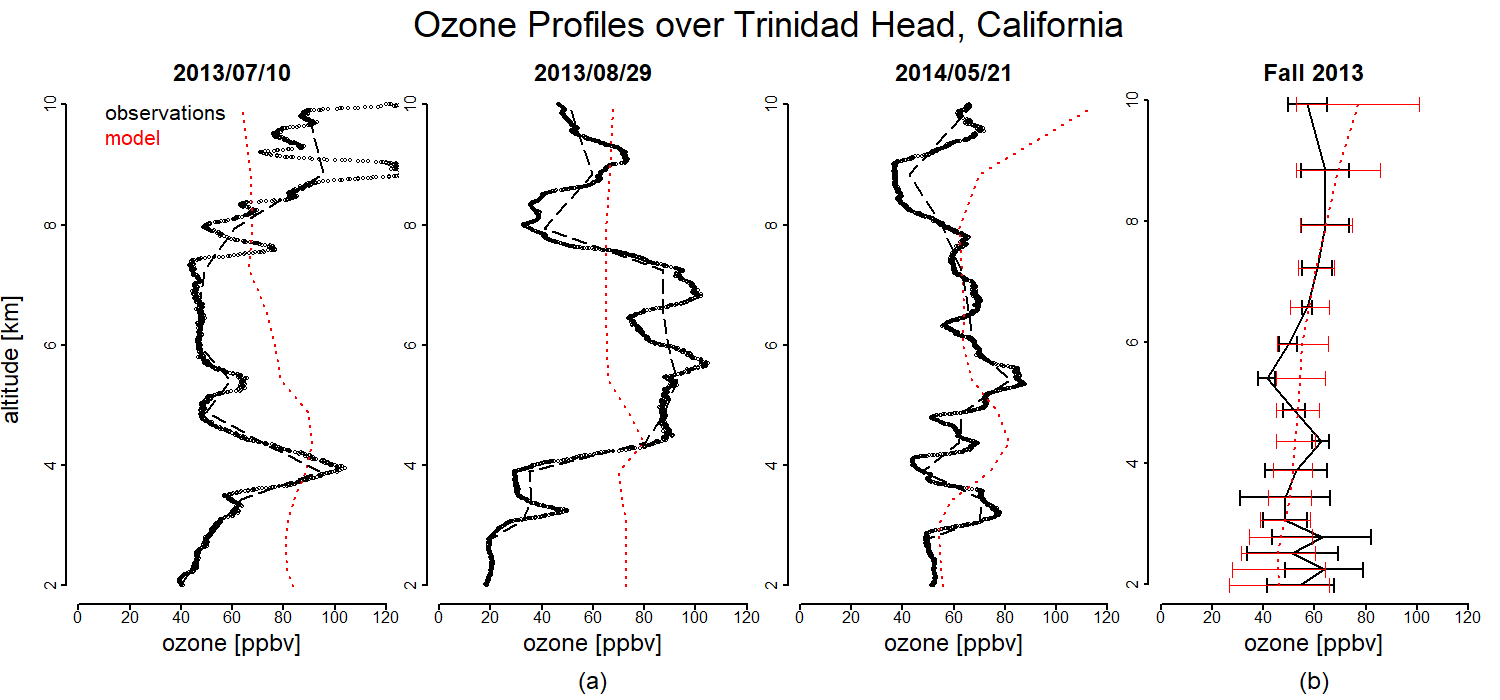
\includegraphics[width=10cm,height=6cm,keepaspectratio]{proposal}
\caption{Vertical profiles of ozone over Trinidad Head, California. Ozonesonde observations are compared to GEOS model values. The left panels show three sample vertical profiles during fall 2013 and the right panel shows the seasonal averages (with standard deviations). Also shown as dashed lines in the left panels are the ozonesonde observations averaged over  the vertical resolution of the  GEOS model.}
\label{fig:proposal}
\end{figure}
Here I propose to develop the capability for modeling the global-scale transport of chemical plumes by using a new on-line version of the GEOS-Chem global model of atmospheric composition coupled to the GEOS GCM. My work will take advantage of the long-standing collaboration of the Harvard Atmospheric Chemistry Modeling Group and the NASA Global Modeling and Assimilation Office (GMAO), which manages the GEOS GCM.\\ \\
\textbf{Research Plan:}\\ 
\textbf{1) Determine model resolution requirements to preserve intercontinental plumes}\\
On-line simulation of chemical transport in the GEOS GCM will allow me to experiment with different vertical resolutions maintaining consistency between plume transport and the underlying meteorology. The operational version of the model (c720 in horizontal, 72 layers in vertical) does not preserve the plumes, as illustrated in Figure \ref{fig:proposal}. I will conduct simulations at increasing vertical resolutions with guidance from GEOS GCM scientists. This may require adjustment to convective and radiative parameterizations. \cite{delane} Increasing vertical resolution should add relatively little computational expense since it will involve only the free troposphere and will not incur Courant number limitations.\cite{zhuang} 

I will begin by simulating chemically inert plumes to facilitate interpretation, as the exact solution (preservation of the mixing ratio) is known in that case. I will examine the dissipation of plumes released in different regions of the world, testing in particular the role of wind shear. From these analyses I will derive an optimal vertical resolution for the GEOS GCM that balances plume preservation and computational cost. This will provide the basis for my first Ph.D. publication. 
\\\textbf{2) Evaluate model with atmospheric observations of intercontinental plumes}\\
Building on the resolution requirements inferred above, I will run the on-line GEOS-Chem simulation within the GEOS GCM to test the simulation of observed chemically reactive plumes. My initial focus will be on transpacific plumes transported to North America, for which we have extensive observations from satellites, aircraft, and ozonesondes.  Satellites provide dense mapping of the horizontal extent and day-to-day movement of the plumes but with limited vertical resolution. I plan to use the particularly dense data sets available from IASI for carbon monoxide (CO) and from MODIS for aerosols. Aircraft and ozonesondes complement the satellite data by providing detailed vertical information. I plan to use ozonesonde data from sites across the Pacific in addition to Trinidad Head, and weekly aircraft profiles over the San Francisco Bay area from the AJAX program.\cite{yates} Successful simulation of real-world plumes will have tremendous impact for the credibility of global models to describe intercontinental pollution. This will be the basis for my second PhD publication. \\
 \textbf{3) Assess the implications for nonlinear ozone chemistry}\\
Tropospheric ozone is of central environmental interest as a strong oxidant, radiative forcing agent, and pollutant in surface air. It is produced by photochemical oxidation of CO and hydrocarbons in the presence of nitrogen oxides.\cite{jacob1999} Its lifetime in the free troposphere is several weeks, allowing intercontinental transport to affect ozone air quality in continents downwind.The dependence of ozone production on its precursors is strongly non-linear. Coarse-resolution global model studies have been used to estimate Asian ozone pollution influence over North America  but likely have large errors.\cite{lin} \cite{goldstein} I will examine the sensitivity of the ozone simulation to model resolution within my on-line GEOS-Chem simulation framework, starting from the high resolution needed to preserve intercontinental plumes, and conclude as to the extent of error caused by using coarse resolution. Aitken’s convergence method may be useful to diagnose this numerical error and the rate of convergence as resolution increases. I expect the results to have important implications not only for transpacific pollution but more generally for our understanding of the global tropospheric ozone budget2 This will be the basis for my third PhD publication. \\ \\
\textbf{Expected Implications:}\\
This work will significantly increase current capabilities for representing intercontinental plumes in global atmospheric models. As Earth System Models (ESMs) increasingly incorporate atmospheric chemistry in their integrated simulation of the climate system, our work will define the resolution needed – which may be very different from the resolution required by dynamics.  This may call for conducting dynamical and chemical simulations on different grids.  Our application to transpacific pollution plumes will have direct policy implications by quantifying the extent to which Asian pollution may compromise the ability of the western US to meet air quality standards. 

{\footnotesize
\bibliography{ref}}




\end{document}
